% =====================================================================
%  第 6 章 形变量子化 —— ch06a（§6.1–§6.2）
%  页段：PDF 298–313（原书 p.297–312）
% =====================================================================

% [原文 p.297]
\chapter{形变量子化}

本章讨论形变量子化的代数理论。这一理论把量子可观测量的运算看作经典可观测量的形式形变。形变量子化的研究始于巴延–弗拉托–弗伦斯达尔–利赫内罗维奇–施特恩海默（Bayen–Flato–Frønsdal–Lichnerowicz–Sternheimer）[3] 在 1978 年的开创性工作。在这一理论中，普朗克常数 $\hbar$ 被当作形式变量，用来参数化一族量子代数。一个引人注目的特点是：按孔采维奇 [37] 的定理，形变量子化在任意泊松流形上都存在。这大大扩展了量子化的范围，超出了通常的相空间。

\section{形变量子化}

\subsection{形式形变}

我们固定一个基域，具体情形下取哪个域可从上下文看出。

\begin{definition}{6.1.1}
  设 $\mathbb{V}$ 是向量空间。我们用 $\mathbb{V}[[\lambda]]$ 记系数在 $\mathbb{V}$ 中的 $\lambda$ 的形式幂级数
  \[
  \mathbb{V}[[\lambda]]:=\left\{\sum_{i=0}^\infty a_i\lambda^i
  \;\middle|\; a_i\in\mathbb{V}\right\},
  \]
  并用 $\mathbb{V}((\lambda))$ 记形式洛朗级数
  \[
  \mathbb{V}((\lambda)):=\left\{\sum_{i=N}^\infty a_i\lambda^i
  \;\middle|\; a_i\in\mathbb{V},\ N\in\Z\right\}.
  \]
  当 $\mathbb{V}=R$ 是环时，$R[[\lambda]]$ 与 $R((\lambda))$ 通过
  \[
  \left(\sum a_i\lambda^i\right)\left(\sum b_j\lambda^j\right)
  =\sum_k\left(\sum_{i+j=k}a_ib_j\right)\lambda^k
  \]
  继承良定义的环结构。
\end{definition}

\begin{definition}{6.1.2}
  设 $(A,\cdot)$ 是结合代数。$A$ 的一个形式形变是 $A[[\lambda]]$ 上的结合乘积 $*$，使得

  ① $*$ 是 $\lambda$ 双线性的，即
  \[
  (f(\lambda)a)*b=a*(f(\lambda)b)=f(\lambda)(a*b)
  \]
  对任意 $a,b\in A[[\lambda]]$ 与形式幂级数 $f(\lambda)$。

% [原文 p.298]
  ② 对任意 $a,b\in A$，
  \[
  a*b=a\cdot b+\sum_{k=1}^\infty\lambda^k\mu_k(a,b),
  \]
  其中 $a\cdot b$ 是 $A$ 中的乘积，$\mu_k:A\times A\to A$ 是双线性映射。
\end{definition}

条件 ① 中的 $\lambda$ 线性要求意味着 $*$ 完全由条件 ② 中的 $\{\mu_k\}$ 决定。我们可以把 $*$ 看作定义了以 $\lambda$ 为参数的一族结合乘积，使得
\[
\lim_{\lambda\to0}a*b=a\cdot b.
\]
于是 $*$ 成为结合乘积 $\cdot$ 的形式形变。之所以称为形式形变，是因为我们只考虑关于 $\lambda$ 的形式幂级数，忽略解析性质。解析性质其实很有趣也很重要，但在当前讨论中无关。

\begin{example}{6.1.3}
  考虑相空间 $\R^{2n}$ 上光滑函数的环 $C^\infty(\R^{2n})$。则 Moyal 乘积
  \[
  f*g=f\,e^{\frac{\lambda}{2}\sum_i\left(
  \frac{\overleftarrow{\pa}}{\pa x^i}\frac{\overrightarrow{\pa}}{\pa p_i}
  -\frac{\overleftarrow{\pa}}{\pa p_i}\frac{\overrightarrow{\pa}}{\pa x^i}\right)}g
  \qquad(\lambda=i\hbar)
  \]
  给出 $C^\infty(\R^{2n})$ 的一个形式形变。这里
  \[
  \mu_k(f,g)=\frac{1}{k!}\left(\frac{1}{2}\right)^k
  f\left[\sum_i\left(
  \frac{\overleftarrow{\pa}}{\pa x^i}\frac{\overrightarrow{\pa}}{\pa p_i}
  -\frac{\overleftarrow{\pa}}{\pa p_i}\frac{\overrightarrow{\pa}}{\pa x^i}\right)\right]^k g.
  \]
\end{example}

\begin{example}{6.1.4}
  上例可推广到形式幂级数环 $\R[[x^i,p_i]]$。用 Moyal 乘积的同一公式
  \[
  f\,e^{\frac{\lambda}{2}\sum_i\left(
  \frac{\overleftarrow{\pa}}{\pa x^i}\frac{\overrightarrow{\pa}}{\pa p_i}
  -\frac{\overleftarrow{\pa}}{\pa p_i}\frac{\overrightarrow{\pa}}{\pa x^i}\right)}g
  \]
  给出 $\R[[x^i,p_i]]$ 的一个形式形变。
\end{example}

$*$ 的结合性要求给出双线性映射 $\{\mu_k\}$ 的一组约束。例如在 $\lambda$ 的一阶，
\[
\begin{aligned}
&(a*b)*c-a*(b*c)\\
&=\big(a\cdot b+\mu_1(a,b)\lambda\big)*c-a*\big(b\cdot c+\mu_1(b,c)\lambda\big)\\
&\qquad+O(\lambda^2)\\
&=(a\cdot b)\cdot c+\lambda\big(\mu_1(a\cdot b,c)+\mu_1(a,b)\cdot c\big)\\
&\qquad-a\cdot(b\cdot c)-\lambda\big(\mu_1(a,b\cdot c)+a\cdot\mu_1(b,c)\big)+O(\lambda^2)\\
&=\lambda\big(\mu_1(a\cdot b,c)+\mu_1(a,b)\cdot c-\mu_1(a,b\cdot c)-a\cdot\mu_1(b,c)\big)+O(\lambda^2).
\end{aligned}
\]
这里最后一步用了未形变乘积 $\cdot$ 的结合性。因此 $\mu_1$ 必须满足如下方程
\[
a\cdot\mu_1(b,c)-\mu_1(a\cdot b,c)+\mu_1(a,b\cdot c)-\mu_1(a,b)\cdot c=0.
\]
我们指出，这其实是霍赫希尔德上同调中的上闭链条件。

% [原文 p.299]
\subsection{泊松代数作为经典极限}

\begin{definition}{6.1.5}
  泊松代数是指交换代数 $P$ 配以双线性映射（称为泊松括号）
  \[
  \{-,-\}:P\times P\longrightarrow P,
  \]
  满足以下性质：对任意 $a,b,c\in P$，

  ① 反对称性：$\{a,b\}=-\{b,a\}$；

  ② 莱布尼茨法则：$\{a,bc\}=\{a,b\}c+b\{a,c\}$；

  ③ 雅可比恒等式：$\{a,\{b,c\}\}+\{b,\{c,a\}\}+\{c,\{a,b\}\}=0$。

  注意由反对称性，莱布尼茨法则对第一个因子也成立
  \[
  \{ab,c\}=a\{b,c\}+\{a,c\}b.
  \]
\end{definition}

\begin{example}{6.1.6}
  设 $M$ 是辛流形。则
  \[
  (C^\infty(M),\{-,-\})
  \]
  是泊松代数。这里 $\{-,-\}$ 是与辛结构相伴的泊松括号。换言之，经典可观测量构成一个泊松代数。
\end{example}

设 $(A,\cdot)$ 是交换代数，$(A[[\lambda]],*)$ 是 $A$ 的形式形变。记
\[
[a,b]_*:=a*b-b*a
\]
为关于乘积 $*$ 的交换子。由于 $*$ 结合，$[-, -]_*$ 满足雅可比恒等式
\[
[a,[b,c]_*]_*+[b,[c,a]_*]_*+[c,[a,b]_*]_*=0
\]
（练习：验证之。）因此 $[-, -]_*$ 定义了 $A[[\lambda]]$ 上的李括号，它衡量 $*$ 的非交换性。
由未形变代数 $(A,\cdot)$ 的交换性，对任意 $a,b\in A$ 有
\[
[a,b]_*=\lambda(\mu_1(a,b)-\mu_1(b,a))+O(\lambda^2).
\]
我们定义 $\{-,-\}:A\times A\longrightarrow A$ 为
\[
\{a,b\}:=\mu_1(a,b)-\mu_1(b,a),
\]
或写成
\[
\{a,b\}=\lim_{\lambda\to0}\frac{1}{\lambda}(a*b-b*a),
\]
它刻画了 $*$ 的一阶非交换性。

\begin{proposition}{6.1.7}
  $(A,\cdot,\{-,-\})$ 构成泊松代数。
\end{proposition}

% [原文 p.300]
\begin{proof}
  反对称性显然。莱布尼茨法则来自
  \[
  \frac{1}{\lambda}\big([a,b*c]_*-[a,b]_**c-b*[a,c]_*\big)=0
  \]
  的 $\lambda\to0$ 极限。雅可比恒等式来自
  \[
  \frac{1}{\lambda^2}\big([a,[b,c]_*]_*+[b,[c,a]_*]_*+[c,[a,b]_*]_*\big)=0
  \]
  的 $\lambda\to0$ 极限。
\end{proof}

我们可以把上面的讨论概括为
\[
\text{结合代数的 }\lambda\text{ 族}\ \xrightarrow{\ \lambda\to0\ }\ \text{泊松代数}.
\]
在力学问题中，我们通常有一个经典系统，其经典可观测量构成泊松代数。形变量子化的纲领要求构造量子化代数 $(A[[\lambda]],*)$，使它的经典极限恰为预先给定的泊松代数（$\lambda=i\hbar$）：
\begin{center}
\begin{tikzpicture}[>=Stealth,scale=0.95]
\node (P) at (0,0) {泊松代数};
\node (A) at (5.4,0) {结合代数};
\draw[->] ([yshift=1.6mm]P.east) -- ([yshift=1.6mm]A.west)
  node[midway,above] {量子化};
\draw[->] ([yshift=-1.6mm]A.west) -- ([yshift=-1.6mm]P.east)
  node[midway,below] {经典极限};
\end{tikzpicture}
\end{center}
% [图：原书 p.300，本图按原文重绘，图内标注已译为中文；原图无题注]

\begin{definition}{6.1.8}
  泊松代数 $(A,\cdot,\{-,-\})$ 的（形式）形变量子化是指形式形变 $(A[[\lambda]],*)$，使得
  \[
  \{-,-\}=\lim_{\lambda\to0}\frac{1}{\lambda}[-, -]_*.
  \]
\end{definition}

给定泊松代数，其形变量子化可能不唯一。

\begin{example}{6.1.9}
  取 $A=C^\infty(\R^2)$，
  \[
  \{f,g\}=\frac{\pa f}{\pa x}\frac{\pa g}{\pa p}-\frac{\pa f}{\pa p}\frac{\pa g}{\pa x}.
  \]
  设 $*$ 是标准 Moyal 乘积
  \[
  f*g=f\,e^{\frac{\lambda}{2}\left(
  \frac{\overleftarrow{\pa}}{\pa x}\frac{\overrightarrow{\pa}}{\pa p}
  -\frac{\overleftarrow{\pa}}{\pa p}\frac{\overrightarrow{\pa}}{\pa x}\right)}g.
  \]
  对任意 $\alpha\in\R$，考虑算子
  \[
  N_\alpha:=e^{\frac{\lambda}{2}\alpha\frac{\pa}{\pa x}\frac{\pa}{\pa p}}:
  A[[\lambda]]\longrightarrow A[[\lambda]].
  \]
  这里 $e^{\frac{\lambda}{2}\alpha\frac{\pa}{\pa x}\frac{\pa}{\pa p}}$ 按其幂级数展开理解。$N_\alpha$ 可逆，且 $N_\alpha^{-1}=N_{-\alpha}$。我们定义
  \[
  f*_\alpha g:=N_\alpha^{-1}\big((N_\alpha f)*(N_\alpha g)\big).
  \]
  显然对任意 $\alpha\in\R$，$(A[[\lambda]],*_\alpha)$ 定义了形式形变。显式地，
  \[
  f*_\alpha g=f\,e^{\frac{\lambda}{2}\left[
  (1-\alpha)\frac{\overleftarrow{\pa}}{\pa x}\frac{\overrightarrow{\pa}}{\pa p}
  -(1+\alpha)\frac{\overleftarrow{\pa}}{\pa p}\frac{\overrightarrow{\pa}}{\pa x}\right]}g.
  \]
  特别地，
  \[
  \{f,g\}=\lim_{\lambda\to0}\frac{1}{\lambda}(f*_\alpha g-g*_\alpha f)
  \]

% [原文 p.301]
  对任意 $\alpha\in\R$ 成立。因此对任意 $\alpha\in\R$，$(A[[\lambda]],*_\alpha)$ 是 $(A,\cdot,\{-,-\})$ 的形变量子化。当 $\alpha=0$ 时得到 Moyal 乘积。当 $\alpha=1$ 时，
  \[
  f*_1g=f\,e^{\left(-\lambda\frac{\overleftarrow{\pa}}{\pa p}
  \frac{\overrightarrow{\pa}}{\pa x}\right)}g,
  \]
  与正规序有关：它把量子算子 $\wh p=-\lambda\frac{\pa}{\pa x}$ 放在 $x$ 的右边，
  \[
  x*_1p=xp,\qquad p*_1x=xp-\lambda.
  \]
  因此 $*_{\alpha=1}$ 刻画了微分算子的复合。
\end{example}

\subsection{严格形变量子化}

里费尔（Rieffel）[49, 50] 引入了严格形变量子化的概念，为把量子化理解为经典系统到量子系统的连续形变提供了数学框架。这些形变量子化之所以是「严格」的，是因为它们给出的是以实参数 $\hbar$（普朗克常数）为参数的连续 $C^*$ 代数族，而不是形式幂级数。

\begin{definition}{6.1.10}
  泊松流形 $M$ 的严格形变量子化由以下数据组成：某个包含 $0$ 的区间 $I\subseteq\R$ 上的连续 $C^*$ 代数场 $\{A_\hbar\}_{\hbar\in I}$，其中 $A_0=C_0(M)$（$M$ 上无穷远处趋于零的连续函数构成的交换 $C^*$ 代数）；以及对每个 $\hbar\in I$ 的线性映射 $Q_\hbar:C_c^\infty(M)\to A_\hbar$，满足：
  \begin{enumerate}[label=\arabic*.,leftmargin=2.2em,itemsep=0.2em]
  \item 对每个 $f\in C_c^\infty(M)$，映射 $\hbar\mapsto Q_\hbar(f)$ 是该场的连续截面。
  \item $Q_0$ 是 $C_c^\infty(M)$ 到 $C_0(M)$ 的典范包含。
  \item 对 $f,g\in C_c^\infty(M)$，如下狄拉克条件成立：
  \[
  \lim_{\hbar\to0}\left\|\frac{i}{\hbar}[Q_\hbar(f),Q_\hbar(g)]
  -Q_\hbar(\{f,g\})\right\|=0,
  \]
  其中 $\{f,g\}$ 是泊松括号。
  \item 对每个 $\hbar\in I$，映射 $Q_\hbar$ 在 $A_\hbar$ 中的像稠密。
  \end{enumerate}
\end{definition}

\begin{example}{6.1.11}
  设 $M=\R^{2n}$ 是标准相空间。则外尔量子化与 Moyal 乘积实际上给出一个严格形变量子化。
\end{example}

\begin{example}{6.1.12}
  设 $M=\mathbb{T}^n$ 是 $n$ 维环面。令 $A_0=C(\mathbb{T}^n)$，$\Theta$ 是实反对称 $n\times n$ 矩阵。非交换环面 $A_\Theta$（或量子环面）由满足
  \[
  U_jU_k=e^{2\pi i\Theta_{jk}}U_kU_j
  \]
  的酉元 $U_1,\cdots,U_n$ 生成。
  若令 $\Theta=\hbar\Theta_0$ 并令 $\hbar\to0$，我们回到交换环面 $C(\mathbb{T}^n)$，而族 $A_{\hbar\Theta_0}$ 构成 $C(\mathbb{T}^n)$ 的某个合适稠密子代数的严格形变量子化。
\end{example}

本讲义余下部分，我们专注于一般存在性与显式构造都已知的形式形变量子化。

\takeaway{本节把形变量子化定义为结合乘积关于形式参数 $\lambda$ 的形变：Moyal 乘积给出相空间上的基本例子，结合性的一阶条件引出霍赫希尔德上闭链；形变参数趋零时的交换子给出泊松括号，故经典极限是泊松代数。严格形变量子化则把形式幂级数换成以 $\hbar$ 为参数的连续 $C^*$ 代数族。}

% [原文 p.302]
\section{辛流形上的几何进路}

设 $(M,\omega)$ 是 $2n$ 维辛流形。相空间 $M$ 上的经典可观测量构成泊松代数 $(C^\infty(M),\{-,-\})$。德维尔德–勒孔特（DeWilde–Lecomte）[14] 在 1983 年用上同调方法得到了辛流形上形变量子化的一般存在性。独立地，费多谢夫（Fedosov）[19] 在 1985 年用微分几何方法给出了另一条漂亮的进路。
本节我们讲述费多谢夫在辛流形上构造形变量子化的几何方法。基本想法是：局部地，$(M,\omega)$ 以标准辛空间 $\R^{2n}$ 为模型，而在那里外尔量子化可用。于是我们可以用相容的平行移动（即用一个平坦联络）把这些局部量子化粘成整体的量子化。

\subsection{外尔丛}

\textbf{形式外尔代数}

设 $(V,\omega)$ 是 $2n$ 维线性辛空间。记
\[
\widehat{\mathcal{O}}(V):=\prod_{k=0}^\infty\Sym^k(V^*),
\qquad V^*=\Hom_\R(V,\R)
\]
为 $V$ 上形式幂级数之环。设 $\{e_1,\cdots,e_{2n}\}$ 是 $V$ 的线性基，
\[
\omega_{ij}:=\omega(e_i,e_j).
\]
设 $\{y^1,\cdots,y^{2n}\}$ 是 $V^*$ 的对偶基，可视为 $V$ 上的一组线性坐标。于是可以把
\[
\widehat{\mathcal{O}}(V):=\R[[y^i]]
\]
等同起来，并把辛形式写成
\[
\omega=\frac{1}{2}\sum_{i,j=1}^{2n}\omega_{ij}dy^i\wedge dy^j.
\]
$\widehat{\mathcal{O}}(V)$ 上的泊松括号为
\[
\{f,g\}=\sum_{i,j}\omega^{ij}\pa_{y^i}f\pa_{y^j}g,
\]
其中 $\omega^{ij}$ 是 $\omega_{ij}$ 的逆矩阵。

\begin{definition}{6.2.1}
  我们定义与线性辛空间 $(V,\omega)$ 相伴的形式外尔代数 $\mathcal{W}(V)$ 为
  \[
  \mathcal{W}(V)=\left(\widehat{\mathcal{O}}(V)[[\lambda]],*\right),
  \]
  其中对 $f,g\in\widehat{\mathcal{O}}(V)[[\lambda]]$，
  \[
  f*g:=f\,e^{\frac{\lambda}{2}\sum_{i,j}\omega^{ij}
  \frac{\overleftarrow{\pa}}{\pa y^i}
  \frac{\overrightarrow{\pa}}{\pa y^j}}g.
  \]
  这里为简单起见省略了 $\mathcal{W}(V)$ 对线性辛形式 $\omega$ 的依赖。上述 $*$ 的定义不依赖线性坐标的选取。显然 $\mathcal{W}(V)$ 给出 $\left(\widehat{\mathcal{O}}(V),\{-,-\}\right)$ 的形变量子化。
\end{definition}

% [原文 p.303]
\textbf{外尔丛}

设 $(M,\omega)$ 是 $2n$ 维辛流形。对任意 $p\in M$，
\[
(T_pM,\omega|_{T_pM})
\]
定义线性辛空间。

\begin{center}
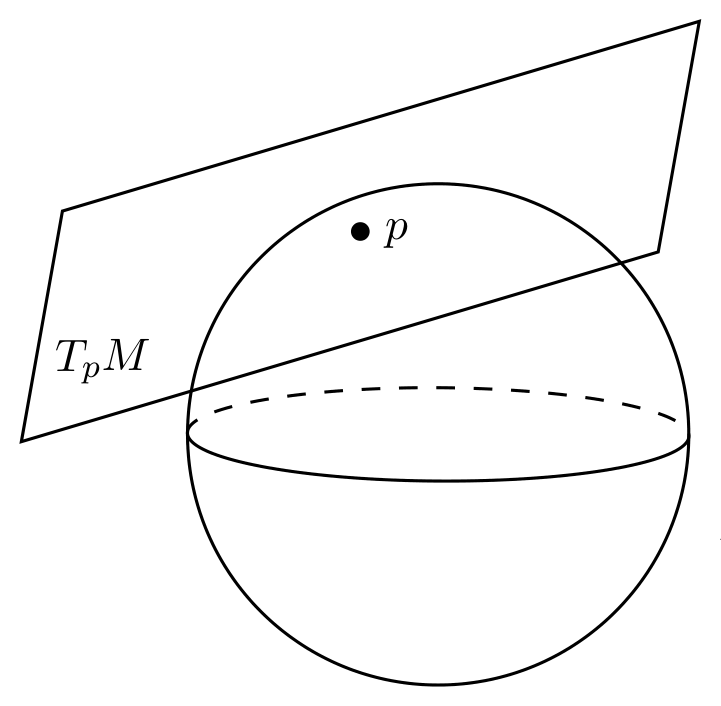
\includegraphics[width=0.65\textwidth]{figures/fig_p304_a.png}
\end{center}
% [图：原书 p.303，图内文字照原样保留；原图无题注]

设 $\mathcal{W}(T_pM)$ 是与线性辛空间 $(T_pM,\omega|_{T_pM})$ 相伴的形式外尔代数。这可看作在点 $p\in M$ 附近局部化的量子化。

\begin{definition}{6.2.2}
  $(M,\omega)$ 的\textbf{外尔丛}定义为
  \[
  \mathcal{W}(M):=\prod_{k=0}^\infty\Sym^k(T^*M)[[\lambda]].
  \]
  外尔丛的秩为无穷。在每点 $p\in M$，$\mathcal{W}(M)$ 在 $p$ 的纤维是
  \[
  \mathcal{W}(M)|_p=\mathcal{W}(T_pM).
  \]
  更确切地说，$\mathcal{W}(M)$ 的光滑截面 $s$ 局部地由
  \[
  s(\mathbf x,\mathbf y,\lambda)
  =\sum_{\substack{k\ge0,\,l\ge0\\ i_1,\cdots,i_l\ge0}}
  \lambda^k a_{k,i_1\cdots i_l}(\mathbf x)y^{i_1}\cdots y^{i_l}
  \]
  给出，其中 $\{a_{k,i_1\cdots i_l}(\mathbf x)\}$ 是定义在 $M$ 的局部坐标
  $\{x^i\}$ 中的光滑函数，$\{y^i\}$ 是 $TM$ 上诱导的纤维坐标。
\end{definition}

为简单起见，当底流形 $M$ 在上下文中清楚时，我们就把外尔丛 $\mathcal{W}(M)$ 简记为 $\mathcal{W}$。我们记
\[
\Gamma(U,\mathcal{W})=\{\mathcal{W}\text{ 在开子集 } U \text{ 中的光滑截面}\}
\]
为 $U$ 中的光滑截面。每个纤维 $\mathcal{W}(T_pM)$ 上的 Moyal 乘积定义了 $\mathcal{W}$ 上逐纤维的乘积，我们仍记为 $*$。显式地，对 $\mathcal{W}$ 的任意两个光滑截面 $s_1,s_2$，在上述局部坐标下有
\[
(s_1*s_2)(\mathbf x,\mathbf y,\lambda)
=s_1(\mathbf x,\mathbf y,\lambda)\,
e^{\frac{\lambda}{2}\sum_{i,j}\omega^{ij}(\mathbf x)
\frac{\overleftarrow{\pa}}{\pa y^i}
\frac{\overrightarrow{\pa}}{\pa y^j}}
s_2(\mathbf x,\mathbf y,\lambda).
\]
于是
\[
\{\Gamma(U,\mathcal{W})\mid U\subset M \text{ 为开子集}\}
\]
构成 $M$ 上的结合代数层。

% [原文 p.304]
\subsection{辛联络}

空间 $\Gamma(M,\mathcal{W})$ 构成结合代数，但对形变量子化来说它太大了。我们接下来的目标是构造 $\mathcal{W}$ 上的一个平坦联络（费多谢夫的阿贝尔联络），以削减自由度。由于 $\mathcal{W}$ 是由切丛 $TM$ 的张量搭起来的丛，$TM$ 上任何联络都在 $\mathcal{W}$ 上诱导一个联络。我们先从这样一个联络出发，并在下一小节讨论费多谢夫如何把曲率平凡化。

\begin{definition}{6.2.3}
  设 $(M,\omega)$ 是辛流形。切丛 $TM$ 上的联络 $\nabla$ 称为\textbf{辛联络}，如果
  \begin{itemize}[leftmargin=1.6em,itemsep=0.2em]
  \item[①] $\nabla$ 无挠
  \[
  \nabla_XY-\nabla_YX=[X,Y],\qquad \forall X,Y\in\mathrm{Vect}(M);
  \]
  \item[②] $\nabla$ 与 $\omega$ 相容
  \[
  \nabla\omega=0.
  \]
  \end{itemize}
\end{definition}

辛联络总是存在。为看出这一点，我们在 $M$ 上取一个度量 $g$，并设 $\nabla^g$ 是相伴的列维–奇维塔联络。则按构造 $\nabla^g$ 无挠，但未必与 $\omega$ 相容。我们寻找
\[
\nabla=\nabla^g+\alpha,\qquad \alpha\in\Omega^1(M,\End(TM))
\]
使 $\nabla$ 成为辛联络。记
\[
\nabla_XY=\nabla^g_XY+\alpha(X,Y).
\]
无挠条件要求
\begin{align*}
\nabla_XY-\nabla_YX-[X,Y]
&=\nabla^g_XY+\alpha(X,Y)-\nabla^g_YX-\alpha(Y,X)-[X,Y]\\
&=\alpha(X,Y)-\alpha(Y,X)=0,
\end{align*}
所以我们要求 $\alpha$ 满足
\[
\alpha(X,Y)=\alpha(Y,X).
\]
与 $\omega$ 相容要求
\[
X\omega(Y,Z)=\omega(\nabla_XY,Z)+\omega(Y,\nabla_XZ),
\]
等价于
\[
\omega(\alpha(X,Y),Z)-\omega(\alpha(X,Z),Y)
=X\omega(Y,Z)-\omega(\nabla^g_XY,Z)-\omega(Y,\nabla^g_XZ).
\]
设 $\xi$ 是由
\[
\xi(X,Y,Z)=X\omega(Y,Z)-\omega(\nabla^g_XY,Z)-\omega(Y,\nabla^g_XZ)
\]
定义的张量。

% [原文 p.305]
$\omega$ 的反对称性推出
\[
\xi(X,Y,Z)=-\xi(X,Z,Y).
\]
$\nabla^g$ 的无挠性与 $d\omega=0$ 推出 $\xi$ 的全反对称化消失，即
\[
\xi(X,Y,Z)+\xi(Y,Z,X)+\xi(Z,X,Y)=0.
\]
我们寻找 $\alpha$ 满足
\[
\begin{cases}
\alpha(X,Y)=\alpha(Y,X),\\
\omega(\alpha(X,Y),Z)-\omega(\alpha(X,Z),Y)=\xi(X,Y,Z).
\end{cases}
\]
这样一个 $\alpha$ 可以通过解方程
\[
\omega(\alpha(X,Y),Z)=\frac13\xi(X,Y,Z)+\frac13\xi(Y,X,Z)
\]
找到。$\omega$ 的非退化性保证该方程有唯一解。这样确定的 $\alpha$ 显然满足 $\alpha(X,Y)=\alpha(Y,X)$，并且
\begin{align*}
&\omega(\alpha(X,Y),Z)-\omega(\alpha(X,Z),Y)\\
&=\frac13\left(\xi(X,Y,Z)+\xi(Y,X,Z)-\xi(X,Z,Y)-\xi(Z,X,Y)\right)\\
&=\frac13\left(2\xi(X,Y,Z)-\left(\xi(Y,Z,X)+\xi(Z,X,Y)\right)\right)\\
&=\frac13\left(2\xi(X,Y,Z)+\xi(X,Y,Z)\right)\\
&=\xi(X,Y,Z),
\end{align*}
正如所需。
与黎曼情形不同，辛联络并不唯一。

\begin{theorem}{6.2.4}
  辛流形上的辛联络总是存在。辛联络之集是以 $\Gamma(M,\Sym^3(T^*M))$ 为模型空间的仿射空间。
\end{theorem}

\begin{proof}
  我们已在上文证明辛联络的存在性。设 $\nabla$ 与 $\nabla'$ 是两个辛联络，它们相差
  \[
  \nabla'_XY=\nabla_XY+\alpha(X,Y).
  \]
  无挠性要求 $\alpha(X,Y)=\alpha(Y,X)$。与 $\omega$ 相容要求
  $\omega(\alpha(X,Y),Z)=\omega(\alpha(X,Z),Y)$。设 $\beta$ 表示张量
  \[
  \beta(X,Y,Z):=\omega(\alpha(X,Y),Z).
  \]
  则上述两个条件变为
  \[
  \begin{cases}
  \beta(X,Y,Z)=\beta(Y,X,Z),\\
  \beta(X,Y,Z)=\beta(X,Z,Y),
  \end{cases}
  \]
  这等价于 $\xi$ 的全对称性，即
  \[
  \beta\in\Gamma(M,\Sym^3(T^*M)).
  \]
  \tutornote{上一句原文作 “the total symmetry of $\xi$”，但由 $\beta(X,Y,Z):=\omega(\alpha(X,Y),Z)$ 知此处指 $\beta$，照原文录入。}
\end{proof}

% [原文 p.306]
\begin{definition}{6.2.5}
  设 $\nabla$ 是 $(M,\omega)$ 上的辛联络，$R^\nabla$ 记其曲率：
  \[
  R^\nabla(X,Y)Z=\left(\nabla_X\nabla_Y-\nabla_Y\nabla_X-\nabla_{[X,Y]}\right)Z
  \]
  对 $M$ 上的向量场 $X,Y,Z$。由张量
  \[
  R^\nabla_\omega(X,Y,Z,T):=\omega(R^\nabla(X,Y)Z,T)
  \]
  定义\textbf{辛曲率} $R^\nabla_\omega$。
\end{definition}

与 $\omega$ 相容推出
\begin{align*}
R^\nabla_\omega(X,Y,Z,T)
&=\omega\left(\left(\nabla_X\nabla_Y-\nabla_Y\nabla_X-\nabla_{[X,Y]}\right)Z,T\right)\\
&=-\omega\left(Z,\left(\nabla_X\nabla_Y-\nabla_Y\nabla_X-\nabla_{[X,Y]}\right)T\right)\\
&=-\omega\left(Z,R^\nabla(X,Y)T\right)\\
&=\omega\left(R^\nabla(X,Y)T,Z\right)\\
&=R^\nabla_\omega(X,Y,T,Z).
\end{align*}
因此 $R^\nabla_\omega$ 对前两个变量反对称、对后两个变量对称：
\[
R^\nabla_\omega\in\Gamma\left(M,\bigwedge^2(T^*M)\otimes\Sym^2(T^*M)\right).
\]
由于 $\nabla$ 无挠，$R^\nabla_\omega$ 还满足第一比安基恒等式
\[
R^\nabla_\omega(X,Y,Z,T)+R^\nabla_\omega(Y,Z,X,T)+R^\nabla_\omega(Z,X,Y,T)=0.
\]

\subsection{费多谢夫的阿贝尔联络}

设 $\nabla$ 是 $(M,\omega)$ 上的辛联络。它在所有张量 $\Sym^k(T^*M)$ 上自然诱导一个联络，从而在外尔丛
\[
\mathcal{W}=\prod_{k=0}^\infty\Sym^k(T^*M)[[\lambda]]
\]
上诱导一个联络。
设 $\{x^i\}$ 是 $M$ 上的局部坐标，
\[
\omega=\frac{1}{2}\sum_{i,j}\omega_{ij}(\mathbf x)dx^i\wedge dx^j,
\qquad \omega_{ij}=\omega(\pa_{x^i},\pa_{x^j}).
\]
设 $\{y^i\}$ 是 $TM$ 上相应的纤维坐标。我们可以把辛曲率张量
\[
R^\nabla_\omega\in\Gamma\left(M,\bigwedge^2(T^*M)\otimes\Sym^2(T^*M)\right)
\]
在局部坐标下表示成
\[
R^\nabla_\omega=\frac{1}{4}\sum_{i,j,k,l}R_{ijkl}(\mathbf x)
dx^i\wedge dx^j\otimes y^ky^l.
\]

% [原文 p.307]
其中 $R_{ijkl}$ 对前两个（$ij$）指标反对称、对后两个（$kl$）指标对称。显式的等同是
\[
\omega(\nabla^2(\pa_{x^k}),\pa_{x^l})
=\frac{1}{2}\sum_{i,j}R_{ijkl}dx^i\wedge dx^j.
\]
我们来看 $\nabla$ 在外尔丛 $\mathcal{W}$ 上的曲率是什么样子。在局部坐标中
$y^i$ 与 $\pa_{x^i}$ 对偶，因此
\[
0=\nabla^2\left(\sum_k\pa_{x^k}\otimes y^k\right)
=\sum_k\nabla^2(\pa_{x^k})\otimes y^k+\pa_{x^k}\otimes\nabla^2y^k.
\]
这意味着
\begin{align*}
\sum_k\omega(\pa_{x^k},\pa_{x^l})\nabla^2y^k
&=-\sum_k\omega(\nabla^2(\pa_{x^k}),\pa_{x^l})\otimes y^k\\
&=-\frac{1}{2}\sum_{i,j,k}R_{ijkl}dx^i\wedge dx^j\otimes y^k,
\end{align*}
即
\[
\sum_k\omega_{kl}\nabla^2y^k
=-\frac{1}{2}\sum_{i,j,k}R_{ijkl}dx^i\wedge dx^j\otimes y^k
\]
\[
\Longrightarrow\qquad
\nabla^2y^m=-\frac{1}{2}\sum_{i,j,k,l}\omega^{lm}R_{ijkl}
dx^i\wedge dx^j\otimes y^k.
\]
我们可以用逐纤维 Moyal 乘积的交换子把它写成
\[
\nabla^2y^m=\frac{1}{\lambda}
\left[-\frac{1}{4}\sum_{i,j,k,l}R_{ijkl}dx^i\wedge dx^j\otimes y^ky^l,
y^m\right]_*
=\left[-\frac{1}{\lambda}R^\nabla_\omega,y^m\right]_*.
\]
利用莱布尼茨法则与 Moyal 乘积公式，对 $\mathcal{W}$ 的任意截面 $s$ 我们有
\[
\nabla^2s=\left[-\frac{1}{\lambda}R^\nabla_\omega,s\right]_*,
\]
即外尔丛 $\mathcal{W}$ 上诱导联络 $\nabla$ 的曲率为
\[
\nabla^2=\left[-\frac{1}{\lambda}R^\nabla_\omega,-\right]_*.
\]
这个诱导联络 $\nabla$ 在 $\mathcal{W}$ 上的另一个好性质是它与逐纤维 Moyal 乘积相容：对 $\mathcal{W}$ 的任意两个截面 $s_1,s_2$，
\[
\nabla(s_1*s_2)=(\nabla s_1)*s_2+s_1*\nabla s_2,
\]
即逐纤维 Moyal 乘积 $*$ 是 $\nabla$ 平行的。这来自如下事实：$*$ 是由 $\omega$ 构造的，而 $\omega$ 本身是 $\nabla$ 平行的。
另一方面，我们可以用不来自 $TM$ 上联络的项来修改 $\mathcal{W}$ 上的诱导联络 $\nabla$。具体地说，对取值于外尔丛的任意 $1$-形式
\[
\gamma\in\Omega^1(M,\mathcal{W}),
\]
我们可以由
\[
D=\nabla+\frac{1}{\lambda}[\gamma,-]_*
\]
在 $\mathcal{W}$ 上定义一个新联络 $D$。

% [原文 p.308]
这样的联络也与逐纤维 Moyal 乘积 $*$ 相容：对 $\mathcal{W}$ 的任意两个截面 $s_1,s_2$，
\begin{align*}
D(s_1*s_2)
&=\nabla(s_1*s_2)+\frac{1}{\lambda}[\gamma,s_1*s_2]_*\\
&=\nabla s_1*s_2+s_1*\nabla s_2+\frac{1}{\lambda}[\gamma,s_1]_**
s_2+\frac{1}{\lambda}s_1*[\gamma,s_2]_*\\
&=(Ds_1)*s_2+s_1*Ds_2.
\end{align*}
要点在于：可以找到 $\gamma$ 使 $D$ 成为 $\mathcal{W}$ 上的平坦联络。这是费多谢夫的关键观察，它将使我们能在辛流形上构造形变量子化。为看出这一点，我们先计算 $D=\nabla+\frac1\lambda[\gamma,-]_*$ 的曲率：
\begin{align*}
D^2&=\nabla^2+\frac{1}{\lambda}[\nabla\gamma,-]_*
+\frac{1}{\lambda^2}[\gamma,[\gamma,-]_*]_*\\
&=\nabla^2+\frac{1}{\lambda}[\nabla\gamma,-]_*
+\frac{1}{2\lambda^2}[[\gamma,\gamma]_*,-]_*\\
&=\frac{1}{\lambda}\left[-R^\nabla_\omega+\nabla\gamma
+\frac{1}{2\lambda}[\gamma,\gamma]_*,-\right]_*.
\end{align*}
注意 $\frac12[\gamma,\gamma]_*=\gamma*\gamma$，因为 $\gamma$ 取值于 $1$-形式。于是我们要找
$\gamma\in\Omega^1(M,\mathcal{W})$，使
$-R^\nabla_\omega+\nabla\gamma+\frac1{2\lambda}[\gamma,\gamma]_*$ 落在 $\mathcal{W}$ 的中心，即
\[
-R^\nabla_\omega+\nabla\gamma+\frac{1}{2\lambda}[\gamma,\gamma]_*
\in\Omega^2(M)[[\lambda]].
\]
这样的联络称为\textbf{阿贝尔联络}。
为构造阿贝尔联络 $\gamma$，我们先考虑算子
\[
\delta:\mathcal{W}\longrightarrow\Omega^1(M,\mathcal{W}),
\]
它在局部坐标下由
\[
\delta=\sum_idx^i\frac{\pa}{\pa y^i}
\]
描述。等价地，若记
\[
\gamma_0=\sum_{i,j}\omega_{ij}dx^iy^j\in\Omega^1(M,\mathcal{W}),
\]
则
\[
\delta=\frac{1}{\lambda}[\gamma_0,-]_*.
\]
注意 $\gamma_0$ 是 $\nabla$ 平行的，并且
\[
\nabla\gamma_0+\frac{1}{2\lambda}[\gamma_0,\gamma_0]_*
=\frac{1}{\lambda}\gamma_0*\gamma_0
=\frac{1}{2}\sum_{i,j,k,l}\omega_{ik}dx^i\omega^{kl}\omega_{jl}dx^j
=-\frac{1}{2}\sum_{i,j}\omega_{ij}dx^i\wedge dx^j=-\omega,
\]
即辛形式的相反数。
我们还考虑伴随算子
\[
\delta^*:\Omega^1(M,\mathcal{W})\longrightarrow\Gamma(M,\mathcal{W}).
\]

% [原文 p.309]
它由
\[
\delta^*=\sum_iy^i\iota_{\pa_{x^i}}
\]
定义。
$\delta$ 与 $\delta^*$ 都扩张到任意次形式
\[
\delta:\Omega^p(M,\mathcal{W})\longrightarrow\Omega^{p+1}(M,\mathcal{W}),
\qquad
\delta^*:\Omega^p(M,\mathcal{W})\longrightarrow\Omega^{p-1}(M,\mathcal{W}),
\]
并满足如下霍奇型关系
\[
\delta\delta^*+\delta^*\delta=p+q
\qquad\text{在 } \Omega^p(M,\Sym^q(T^*M))[[\lambda]] \text{ 上}.
\]
特别地，当 $p+q>0$ 时 $\delta$ 是零伦的。这立刻证明如下结果。

\begin{lemma}{6.2.6}
  上同调 $(\Omega^\bullet(M,\mathcal{W}),\delta)$ 集中在 $0$ 次，并且
  \[
  H^\bullet(\Omega^\bullet(M,\mathcal{W}),\delta)
  =H^0(\Omega^\bullet(M,\mathcal{W}),\delta)=C^\infty(M)[[\lambda]].
  \]
\end{lemma}

我们通过赋值
\[
\mathrm{wt}(y^i)=1,\qquad \mathrm{wt}(\lambda)=2
\]
在外尔丛 $\mathcal{W}$ 上定义 $\Z$ 分次的「权」。显然逐纤维 Moyal 乘积保持权。这样的权定义滤链
\[
\mathcal{W}=\mathcal{W}_0\supset\mathcal{W}_1\supset\cdots\supset\mathcal{W}_m\supset\cdots,
\]
其中 $\mathcal{W}_m$ 由权 $\ge m$ 的元素组成。

\begin{theorem}{6.2.7（费多谢夫）}
  给定 $M$ 上任一列闭 $2$-形式 $\{\omega_k\}_{k\ge1}$，存在形如
  \[
  \gamma=\gamma_0+\gamma^+,\qquad \gamma^+\in\Omega^1(M,\mathcal{W}_3)
  \]
  的 $\gamma\in\Omega^1(M,\mathcal{W})$，使得
  \[
  -R^\nabla_\omega+\nabla\gamma+\frac{1}{2\lambda}[\gamma,\gamma]_*
  =\omega_\lambda.
  \]
  这里 $\omega_\lambda=-\omega+\sum_{k\ge1}\lambda^k\omega_k$。特别地，联络
  $D=\nabla+\frac1\lambda[\gamma,-]_*$ 是阿贝尔联络，其在 $\mathcal{W}$ 上的曲率为零。
\end{theorem}

\begin{proof}
  注意 $\frac1\lambda[\gamma_0+\gamma^+,-]_*=\delta+\frac1\lambda[\gamma^+,-]_*$
  且 $\nabla\gamma_0+\frac1{2\lambda}[\gamma_0,\gamma_0]_*=-\omega$。我们记
  \[
  \Sigma(\gamma^+):=\delta\gamma^++\nabla\gamma^+
  +\frac{1}{2\lambda}[\gamma^+,\gamma^+]_*
  -R^\nabla_\omega-\sum_{k\ge1}\lambda^k\omega_k.
  \]
  $\gamma$ 所需的方程为 $\Sigma(\gamma^+)=0$。
  我们把 $\gamma^+$ 分解为
  \[
  \gamma^+=\gamma^+_3+\gamma^+_4+\cdots,
  \]
  其中 $\gamma^+_m$ 是权 $m$ 的齐次分量。注意 $\nabla$ 与 $[-, -]_*$ 都保持权，而
  $\delta$ 把权降低 $1$。我们将按权逐阶求解 $\Sigma(\gamma^+)=0$。

% [原文 p.310]
  $\Sigma(\gamma^+)$ 中权最低的项权为 $2$，我们需要解
  \[
  \delta\gamma^+_3-R^\nabla_\omega-\lambda\omega_1=0.
  \]
  注意由第一比安基恒等式，$\delta(R^\nabla_\omega+\lambda\omega_1)
  =\delta(R^\nabla_\omega)=0$。由引理 6.2.6，$R^\nabla_\omega+\lambda\omega_1$
  必然落在上同调 $2$ 次，故为 $\delta$-恰当的。因此 $\gamma^+_3$ 可解。
  假设已找到
  \[
  \gamma^+_{\le m-1}=\gamma^+_3+\cdots+\gamma^+_{m-1},\qquad m\ge4,
  \]
  使得
  \[
  \Sigma(\gamma^+_{\le m-1})\in\Omega^2(M,\mathcal{W}_{m-1}).
  \]
  我们寻找 $\gamma^+_m$ 使
  \[
  \Sigma(\gamma^+_{\le m})\in\Omega^2(M,\mathcal{W}_m).
  \]
  首先注意对任意 $\gamma$，
  \[
  \left(\nabla+\frac{1}{\lambda}[\gamma,-]_*\right)
  \left(-R^\nabla_\omega+\nabla\gamma+\frac{1}{2\lambda}[\gamma,\gamma]_*\right)=0,
  \]
  这本质上是曲率的比安基恒等式。令
  \[
  \Sigma(\gamma^+_{\le m-1})=\mathcal{O}_{m-1}
  \qquad\text{模 } \Omega^2(M,\mathcal{W}_m),
  \]
  其中 $\mathcal{O}_{m-1}$ 的权为 $m-1$。把上述比安基恒等式应用于
  $\gamma_0+\gamma^+_{\le m-1}$，并利用 $\omega_k$ 闭的事实，得到
  \[
  \Longrightarrow\qquad
  \nabla\Sigma(\gamma^+_{\le m-1})+\delta\Sigma(\gamma^+_{\le m-1})
  +\frac{1}{\lambda}\left[\gamma^+_{\le m-1},
  \Sigma(\gamma^+_{\le m-1})\right]=0.
  \]
  取权最低阶，得到
  \[
  \delta\mathcal{O}_{m-1}=0.
  \]
  另一方面，$\Sigma(\gamma^+_{\le m})$ 的权最低阶为
  \begin{align*}
  \Sigma(\gamma^+_{\le m})
  &=\Sigma(\gamma^+_{\le m-1})+\delta\gamma^+_m
  &&\text{模 } \Omega^2(M,\mathcal{W}_m)\\
  &=\mathcal{O}_{m-1}+\delta\gamma^+_m
  &&\text{模 } \Omega^2(M,\mathcal{W}_m).
  \end{align*}
  由于 $\delta\mathcal{O}_{m-1}=0$ 且 $\mathcal{O}_{m-1}$ 是 $2$-形式，由引理
  6.2.6 知 $\mathcal{O}_{m-1}$ 必为 $\delta$-恰当的。于是我们可以找到
  $\gamma^+_m$ 使 $\mathcal{O}_{m-1}+\delta\gamma^+_m=0$，即
  $\Sigma(\gamma^+_{\le m})\in\Omega^2(M,\mathcal{W}_m)$ 成立。
  于是我们可以递推地构造
  \[
  \gamma=\gamma_0+\gamma^+_3+\gamma^+_4+\cdots+\gamma^+_m+\cdots
  \]
  使得
  \[
  -R^\nabla_\omega+\nabla\gamma+\frac{1}{2\lambda}[\gamma,\gamma]_*
  =\omega_\lambda
  \]
  成立。特别地，$D=\nabla+\frac1\lambda[\gamma,-]_*$ 的曲率为
  \[
  D^2=\frac{1}{\lambda}\left[-R^\nabla_\omega+\nabla\gamma
  +\frac{1}{2\lambda}[\gamma,\gamma]_*,-\right]_*
  =\frac{1}{\lambda}[\omega_\lambda,-]_*=0,
  \]
  因为 $\omega_\lambda$ 落在 $\mathcal{W}$ 的中心。
\end{proof}

% [原文 p.311]
\subsection{象征映射}

设 $D=\nabla+\frac1\lambda[\gamma,-]_*$ 是费多谢夫的阿贝尔联络，它在外尔丛 $\mathcal{W}$ 上给出平坦联络。它定义一个德拉姆链复形
\[
(\Omega^\bullet(M,\mathcal{W}),D),
\]
及其相伴上同调
\[
H^\bullet_D(M,\mathcal{W}):=H^\bullet(\Omega^\bullet(M,\mathcal{W}),D).
\]

\begin{proposition}{6.2.8}
  上同调 $H^\bullet_D(M,\mathcal{W})$ 为
  \[
  H^p_D(M,\mathcal{W})=\begin{cases}
  C^\infty(M)[[\lambda]], & p=0,\\
  0, & p>0.
  \end{cases}
  \]
\end{proposition}

\begin{proof}
  考虑由权诱导的如下滤链
  \[
  F_m\Omega^p(M,\mathcal{W}):=\Omega^p(M,\mathcal{W}_{m-p}).
  \]
  这里对 $k<0$，$\mathcal{W}_k=\mathcal{W}_0=\mathcal{W}$。这给出一个递减滤链
  \[
  \Omega^\bullet(M,\mathcal{W})=F_0\Omega^\bullet(M,\mathcal{W})
  \supset F_1\Omega^\bullet(M,\mathcal{W})\supset\cdots
  \supset F_m\Omega^\bullet(M,\mathcal{W})\supset\cdots
  \]
  费多谢夫的阿贝尔联络具有形式
  \[
  D=\delta+\nabla+\frac{1}{\lambda}[\gamma^+,-]_*,
  \]
  它显然保持 $F_m\Omega^\bullet(M,\mathcal{W})$。分次片上的诱导微分是
  \[
  \delta:\mathrm{Gr}^F_m\longrightarrow\mathrm{Gr}^F_m,
  \qquad
  \mathrm{Gr}^F_m:=\frac{F_m\Omega^\bullet(M,\mathcal{W})}
  {F_{m+1}\Omega^\bullet(M,\mathcal{W})}.
  \]
  由于 $\mathcal{W}$ 由形式幂级数搭成，存在自然的向量空间同构
  \[
  \widehat{\mathrm{Gr}}^F:=\prod_{m\ge0}\mathrm{Gr}^F_m
  \xrightarrow{\ \simeq\ }\Omega^\bullet(M,\mathcal{W}).
  \]
  由引理 6.2.6 推出
  \[
  H^\bullet(\widehat{\mathrm{Gr}}^F,\delta)\simeq
  H^\bullet(\Omega^\bullet(M,\mathcal{W}),\delta)
  =H^0(\Omega^\bullet(M,\mathcal{W}),\delta)=C^\infty(M)[[\lambda]].
  \]
  于是滤链的谱序列在 $E_1$ 页退化，命题得证。
\end{proof}

设 $\Gamma^{flat}_D(M,\mathcal{W})$ 记 $\mathcal{W}$ 的平坦截面空间
\[
\Gamma^{flat}_D(M,\mathcal{W})
:=\{s\in\Gamma(M,\mathcal{W})\mid Ds=0\}.
\]
等价地，我们可以等同
\[
\Gamma^{flat}_D(M,\mathcal{W})=H^0_D(M,\mathcal{W}).
\]

% [原文 p.312]
上述命题说明
\[
0\to\Gamma^{flat}_D(M,\mathcal{W})\to\Omega^0_D(M,\mathcal{W})
\xrightarrow{D}\Omega^1_D(M,\mathcal{W})\xrightarrow{D}\cdots
\]
是正合列，并且
\[
\Gamma^{flat}_D(M,\mathcal{W})\simeq C^\infty(M)[[\lambda]].
\]
这个同构可以显式地描述如下。

\begin{definition}{6.2.9}
  定义\textbf{象征映射}
  \[
  \sigma:\Gamma(M,\mathcal{W})\longrightarrow C^\infty(M)[[\lambda]],
  \qquad
  s(\mathbf x,\mathbf y,\lambda)\mapsto s(\mathbf x,0,\lambda),
  \]
  它把所有纤维变量 $y^i$ 送到零。
\end{definition}

上述谱序列计算表明
\[
\sigma:\Gamma^{flat}_D(M,\mathcal{W})
\xrightarrow{\ \simeq\ }C^\infty(M)[[\lambda]]
\]
给出所需的同构。

\subsection{整体化}

费多谢夫的阿贝尔联络使我们能把局部外尔量子化整体化，得到整个流形上的形变量子化。我们在本小节解释这一构造。
联络 $D=\nabla+\frac1\lambda[\gamma,-]_*$ 与逐纤维 Moyal 乘积相容
\[
D(s_1*s_2)=Ds_1*s_2+s_1*Ds_2.
\]
因此若 $s_1,s_2$ 是平坦截面，$Ds_1=Ds_2=0$，则
\[
D(s_1*s_2)=0,
\]
所以 $s_1*s_2$ 也是平坦截面。于是
\[
(\Gamma^{flat}_D(M,\mathcal{W}),*)
\]
定义结合代数。
借助象征映射给出的同构
\[
\sigma:\Gamma^{flat}_D(M,\mathcal{W})
\xrightarrow{\ \simeq\ }C^\infty(M)[[\lambda]],
\]
我们在 $C^\infty(M)[[\lambda]]$ 上得到诱导的结合乘积 $*_D$
\[
f*_Dg:=\sigma\left(\sigma^{-1}(f)*\sigma^{-1}(g)\right)
\]
对 $f,g\in C^\infty(M)[[\lambda]]$。换言之，象征映射把两个结合代数等同起来
\[
(\Gamma^{flat}_D(M,\mathcal{W}),*)
\xrightarrow{\ \simeq\ }(C^\infty(M)[[\lambda]],*_D).
\]

% [§6.2 的本节重点已移至 ch06b.tex（本节以定理 6.2.10 与其证明结束，在原书 p.313）]

% [块界：本文件译到原书 p.312（PDF 313）页末为止。下一块 ch06b 从原书 p.313 起，]
% [紧接象征映射把两个结合代数等同起来之后的正文继续。]









